\documentclass[11pt]{article}
\usepackage[margin=1in]{geometry}
\usepackage{booktabs}
\usepackage{graphicx}
\usepackage{hyperref}
\usepackage{natbib}

\title{Who Validates the Validators? A Measurement-Science Audit of Benchmark-Validity Diagnostics}
\author{[TO BE FILLED]}
\date{[TO BE FILLED]}

\begin{document}
\maketitle

\begin{abstract}
We present ValidEval, an offline-safe framework for validating benchmark-validity diagnostics before using them to support benchmark claims. The framework pairs controlled flaw injection, diagnostic evidence gates, and claims ledgers with real-data stress tests. In a HELM MMLU / MMLU-Redux stress test, broad matrix-derived diagnostics did not strongly recover documented issue labels, illustrating why diagnostic-specific validation and blocked-claim reporting are necessary.
On a 39-model HELM MMLU panel, we find substantial subject-level ranking sensitivity while proxy diagnostic-weighted rankings remain close to accuracy rankings. Direct/hash MMLU-Redux alignment, decoupled synthetic validation, second-benchmark evidence, and full parametric 2PL remain unresolved gates rather than paper claims.
\end{abstract}

\section{Introduction}

Validity is not accuracy. A benchmark score can be high while the benchmark measures shortcuts,
contamination, scoring artifacts, saturation, or low-discrimination items rather than the claimed
construct.

ValidEval treats benchmark-validity diagnostics as measurement instruments. Diagnostics should
support benchmark claims only after they have evidence about sensitivity, false-positive behavior,
specificity, uncertainty, and materiality under a documented protocol.

The current empirical spine is a public HELM MMLU response matrix with 39 models and 14,042 scored
items. This panel supports artifact-backed analyses of panel validity, proxy psychometric item
diagnostics, subject-level ranking sensitivity, and resampling baselines. The paper treats these
analyses as measurement evidence about diagnostics and rankings, not as a certificate that MMLU is
valid or invalid.

The MMLU-Redux case remains a weak/negative external-validation stress test. Direct or hash-backed
alignment is not confirmed for the current files, and broad matrix-derived diagnostics did not
strongly recover structurally aligned MMLU-Redux labels. The claims ledger therefore blocks
detection-success claims.

The contributions are:

\begin{enumerate}
  \item A measurement-validity framework for benchmark diagnostics with explicit evidence states:
  supported, weak, blocked, or not run.
  \item Artifact-backed real-panel analyses of the active 39-model HELM MMLU matrix, including
  panel validity, proxy IRT diagnostics, subject-level rank sensitivity, and baselines.
  \item A claims-ledger and evidence-gating workflow that prevents unsupported validity claims.
  \item A MMLU-Redux stress test showing that broad proxy diagnostics do not automatically validate
  against structurally aligned external issue labels.
  \item An offline-safe toolkit and reproducible audit artifact format for benchmark authors and
  evaluators.
\end{enumerate}

\section{Related Work}

ValidEval is not another leaderboard runner; it is a diagnostic-validation and claim-gating
framework for benchmark-validity diagnostics.

The framework builds on measurement-validity and psychometric traditions
\citep{messick1995validity,aera2014standards}, but applies them to cached language-model
benchmark artifacts rather than treating a benchmark score as self-interpreting. It complements
evaluation runners such as HELM and lm-evaluation-harness
\citep{liang2022helm,gao2023lmevalharness}: those systems make model evaluation reproducible,
while ValidEval asks what benchmark-validity claims the resulting response matrix can support.

The current artifact spine uses MMLU and MMLU-Redux as a stress test
\citep{hendrycks2021mmlu,gema2024mmlu}. GSM8K, BBH, TruthfulQA, GPQA, and MMLU-Pro are treated
as candidate or deferred benchmark families, not as completed evidence in this draft
\citep{cobbe2021gsm8k,suzgun2022bbh,lin2022truthfulqa,rein2023gpqa,wang2024mmlupro}.

\section{Validity Framework}

Validity is treated as a multidimensional evidence profile rather than a scalar score, following
the measurement principle that score interpretations require evidence for the intended use rather
than only high reliability or high accuracy \citep{messick1995validity,aera2014standards}. A
diagnostic can support a paper claim only when the artifact trail specifies the construct, the
response panel, the scoring rule, the diagnostic family, uncertainty or baseline checks where
available, and the claim boundary.

The framework separates three states that are often conflated. First, a benchmark can have a valid
response matrix for a diagnostic without proving the benchmark measures its intended construct.
Second, a diagnostic can flag suspicious items without proving those items are externally confirmed
errors. Third, a ranking can be sensitive to subjects or item subsets without becoming a true model
ranking. ValidEval records these distinctions in claims ledgers and evidence-state tables.

The active paper evidence uses this gate discipline: the 39-model MMLU panel passes the local
panel-validity gate, proxy IRT diagnostics are available, subject-level rank sensitivity is
artifact-backed, and MMLU-Redux direct/hash validation remains blocked.

\section{The \texttt{valideval} Toolkit}

The toolkit is built around cached response matrices and reproducible artifact directories. For the
MMLU case study, ValidEval imports wide prediction records, builds a model-by-item correctness
matrix, runs a panel-validity gate, computes proxy psychometric item diagnostics, and writes
ranking, subject-instability, diagnostic-disagreement, and baseline artifacts.

The release workflow also includes claim ledgers, blocked-claim reports, paper tables and figures,
Kaggle execution packaging, and reviewer-packet tooling. Scaffolds are kept separate from evidence:
decoupled synthetic validation, second-benchmark runs, full 2PL, and direct/hash MMLU-Redux
alignment remain marked as \texttt{RESULT\_REQUIRED} or blocked unless a saved artifact proves that
the run occurred.

\section{Audit Protocol}

The audit protocol starts by freezing the active evidence state. For this draft, the active MMLU
panel is \texttt{cache/mmlu/wide/matrix.csv}, derived from the HELM wide prediction details. Legacy
three-model MMLU files are retained only as provenance. All analyses are run against cached local
artifacts; no paid API calls or downloads are required for the reported MMLU results.

The protocol then applies gates in order: panel shape and missingness, panel-validity, proxy item
diagnostics, ranking and subject-instability analyses, baseline comparisons, and external validation
attempts. Missing or blocked steps are reported explicitly. In this run, direct/hash MMLU-Redux
alignment is blocked, decoupled synthetic validation is blocked by missing preregistration guard
artifacts, and second-benchmark execution is deferred to the Kaggle package.

\section{Results}

\paragraph{Active panel.} The reconciled active MMLU panel is the 39-model HELM wide matrix with
14,042 scored items and zero missingness. The panel-validity gate passes with ability spread
0.580. Historical three-model files are provenance only, not the active panel.

\begin{figure}[t]
  \centering
  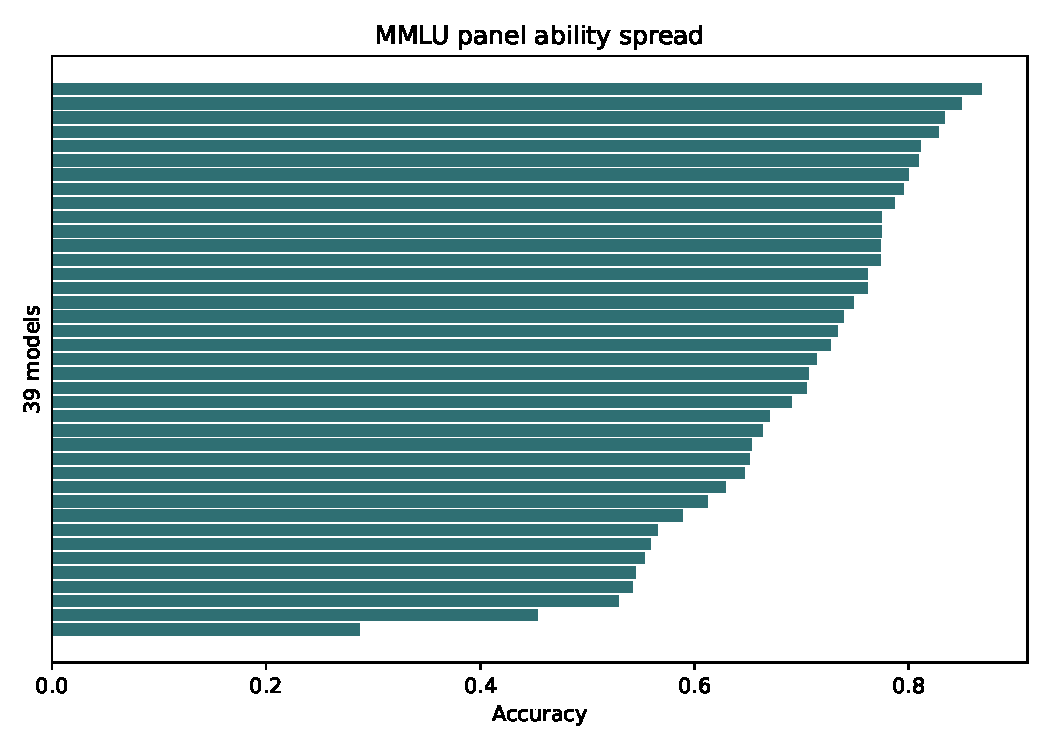
\includegraphics[width=0.78\linewidth]{figures/panel_ability_spread.pdf}
  \caption{Model accuracy spread across the active 39-model HELM MMLU panel.}
\end{figure}

\paragraph{Proxy psychometrics.} Proxy IRT diagnostics were computed for all 14,042 items. The
proxy run flags 1,037 negative-discrimination items, 1,342 near-zero-discrimination items, and
2,676 extreme-difficulty items. Rasch/1PL is not available for this wide matrix under the local BFGS
implementation, and the 2PL run exports proxy slopes only.

\begin{figure}[t]
  \centering
  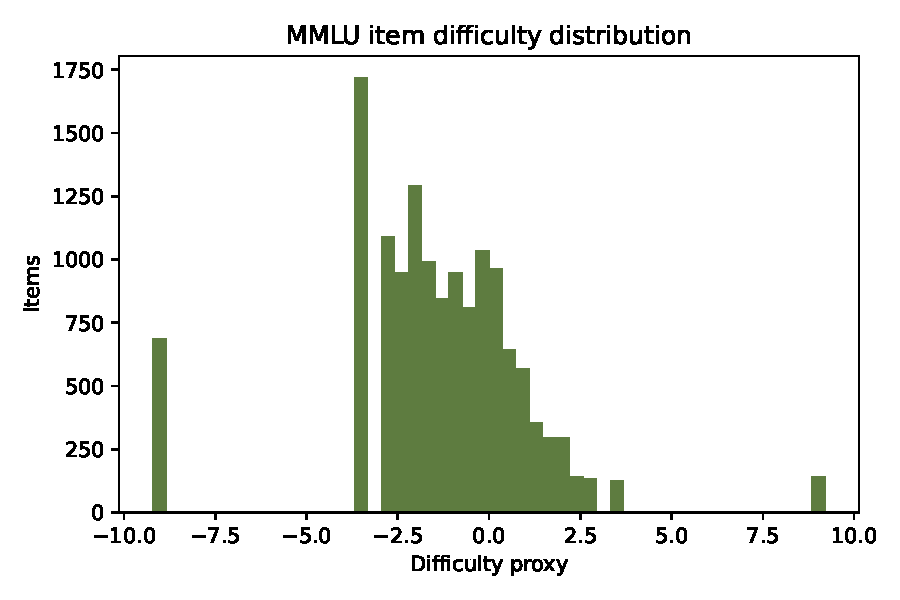
\includegraphics[width=0.48\linewidth]{figures/mmlu_item_difficulty_distribution.pdf}
  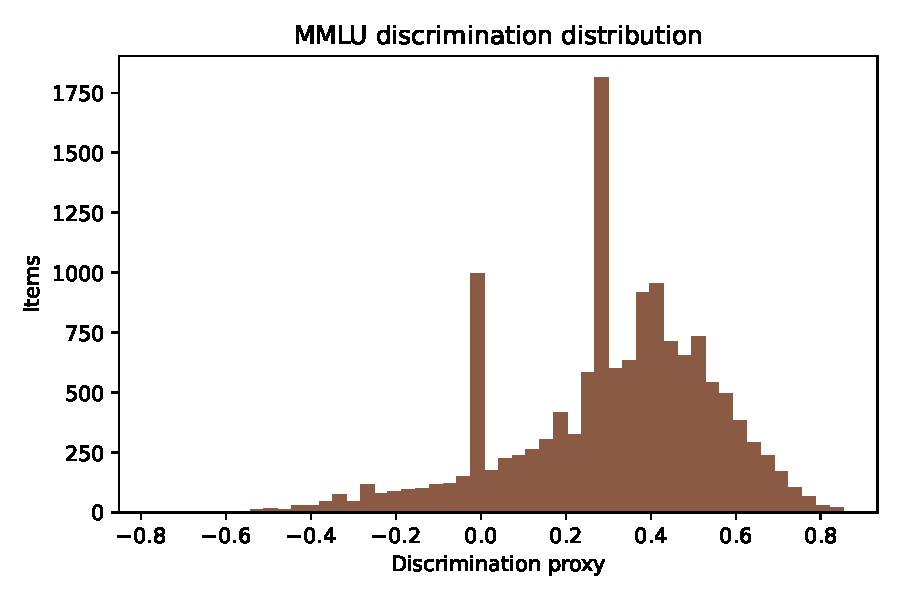
\includegraphics[width=0.48\linewidth]{figures/mmlu_discrimination_distribution.pdf}
  \caption{Proxy item difficulty and discrimination distributions on the active MMLU panel.}
\end{figure}

\paragraph{Ranking sensitivity.} Subject-level ranks vary substantially: every model has subject
rank range at least 3, and the maximum subject rank range is 30. In contrast, proxy
diagnostic-weighted ranking is very close to accuracy ranking, with Spearman correlation 0.998 and
maximum absolute rank delta 2.

\begin{figure}[t]
  \centering
  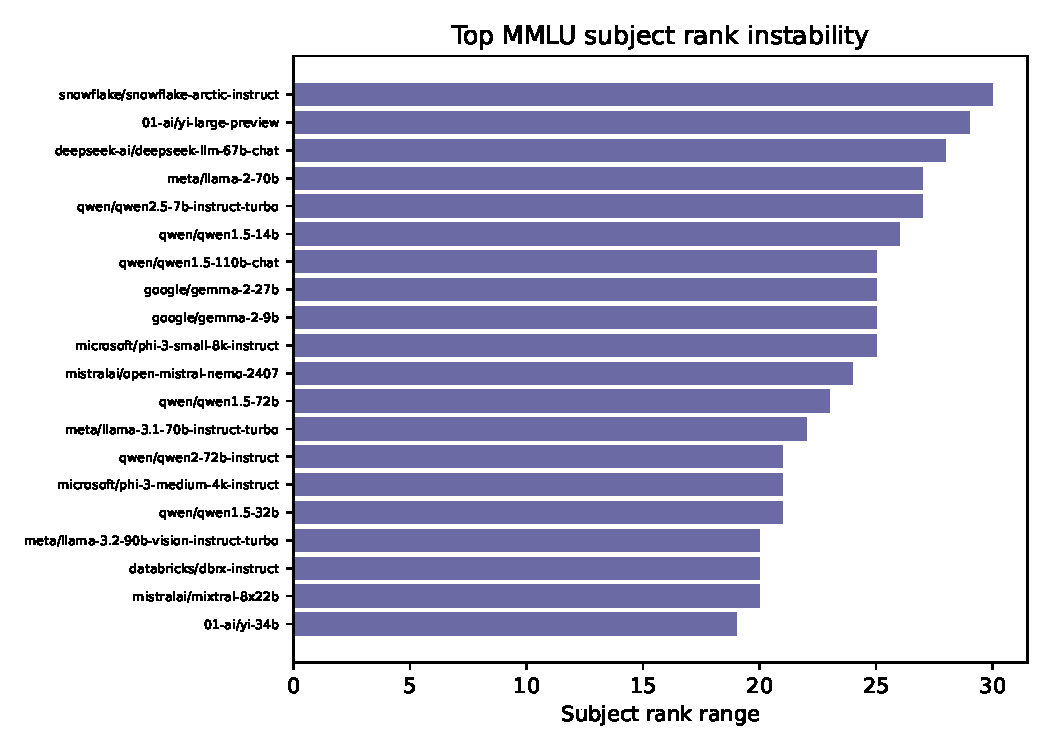
\includegraphics[width=0.48\linewidth]{figures/mmlu_ranking_instability.pdf}
  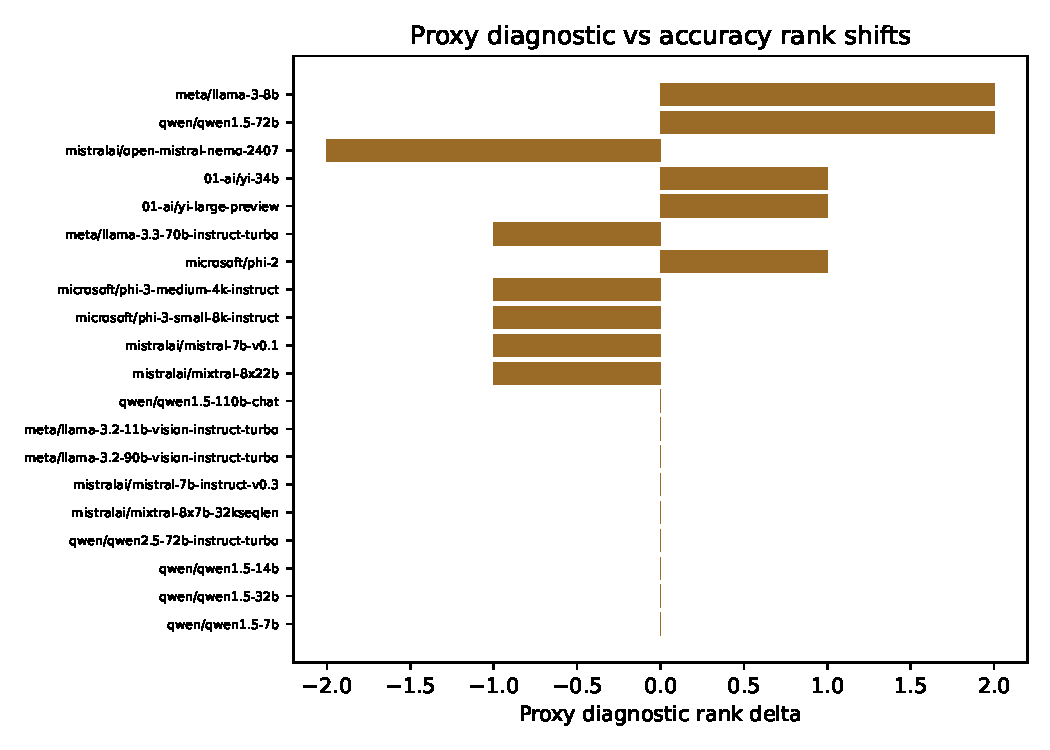
\includegraphics[width=0.48\linewidth]{figures/mmlu_diagnostic_disagreement.pdf}
  \caption{Subject-level rank instability is larger than proxy diagnostic-vs-accuracy rank shifts in this run.}
\end{figure}

\paragraph{Baselines.} Random-item and subject-stratified bootstrap baselines are stable at the top
of the ranking. Across 1,000 iterations per baseline, top-1 match rate is 1.0 and the 95th
percentile max absolute rank delta is 3.0.

\paragraph{MMLU-Redux.} Direct/hash alignment remains blocked: the current files have zero direct
item-id matches and no stable metadata or hash match path. The available structural alignment maps
370 labels by \texttt{subject\_numeric\_index}. Existing structural metrics remain weak/negative
(AUROC 0.539, AUPRC 0.0289, precision@10 0.0), so detection-success claims are blocked.

\paragraph{Deferred evidence.} Decoupled synthetic validation, second-benchmark evidence, Kaggle
output import, full Rasch/1PL, and full parametric 2PL remain \texttt{RESULT\_REQUIRED}.

\begin{table}[t]
  \centering
  \begin{tabular}{lrrl}
    \toprule
    Analysis & Spearman & Max rank delta & Claim state \\
    \midrule
    Proxy diagnostic vs. accuracy & 0.998 & 2 & proxy only \\
    Subject instability & -- & 30 & subject sensitivity \\
    \bottomrule
  \end{tabular}
  \caption{Ranking sensitivity summary. Proxy diagnostic weighting is close to accuracy ranking; subject ranks vary more.}
\end{table}

\section{Analysis}

The evidence is consistent with a measurement-science caution: benchmark validity diagnostics need
their own validation and baselines before they can license benchmark claims. The active MMLU panel is
large enough for the implemented proxy diagnostics, but the external MMLU-Redux stress test remains
weak/negative and structurally aligned rather than direct/hash confirmed.

The ranking result is also deliberately bounded. Subject-level rank sensitivity is large enough to
be paper-relevant, but proxy diagnostic-weighted rankings stay close to accuracy rankings. This
means the current evidence supports a claim about subject sensitivity under one public MMLU panel,
not a claim about the true ordering of models.

The blocked gates are part of the result. Decoupled synthetic validation was not run because guard
artifacts are missing. Second-benchmark validation was not run because no local wide panel exists.
The Kaggle notebook creates an execution path, but evidence remains \texttt{RESULT\_REQUIRED} until
outputs are imported and validated.

\begin{figure}[t]
  \centering
  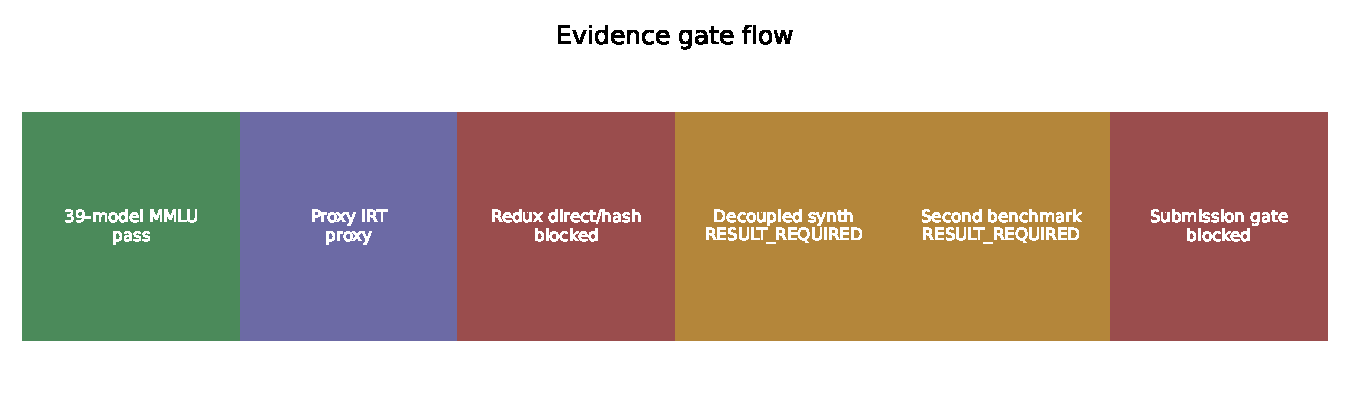
\includegraphics[width=0.82\linewidth]{figures/evidence_gate_flow.pdf}
  \caption{Current evidence gates. Green and purple states are artifact-backed; blocked and result-required states remain claim blockers.}
\end{figure}

\section{Limitations}

MMLU-Redux alignment is structural, using \texttt{subject\_numeric\_index} with confidence 0.85,
not direct-id or hash-confirmed item matching. The MMLU-Redux result is weak/negative external
validation: broad/proxy diagnostics did not strongly recover the structurally aligned labels, and
subject-normalized evidence weakened the earlier raw label-error signal.

The MMLU IRT output is proxy-only and should not be described as full psychometric IRT or full 2PL.
The local Rasch/1PL optimizer is blocked for the active wide matrix because the implementation would
fit 14,080 free parameters; the 2PL output is a proxy-slope export only.
The narrow raw label-error signal is at most a preliminary review-queue cue and does not support
detection-success claims.

Synthetic validation can be circular when generators mirror detectors. The paper should therefore
report the mixed cross-flaw specificity and held-out generator results alongside
false-positive/error-control checks and materiality labels. Synthetic-harness power, numeric
calibration with confidence/logprob outputs, and human-reviewed real-benchmark threshold calibration
remain \texttt{[RESULT REQUIRED]}.

Real benchmark findings remain preliminary and protocol-scoped. The second-benchmark path is
prepared through a Kaggle notebook package, but no Kaggle outputs were imported in this run. Domain
packs are not paper-validated unless separately supported. GPQA local-panel findings are protocol
evidence, not broad validity evidence.

The subject-instability finding may depend on the model panel, HELM extraction, subject taxonomy,
and MMLU item mix. It should be treated as a reproducible panel finding, not a universal property of
all benchmarks or model rankings.

\section{Ethics and Broader Impact}

Validity diagnostics can be misused if their outputs are treated as scalar certificates or as
automatic proof that a benchmark is defective. ValidEval is designed to reduce that risk by pairing
every artifact with a claim state and by preserving blocked results.

The release excludes raw benchmark text from paper-facing artifacts and reviewer packets. Reports use
ids, aggregate metrics, and sanitized tables. This protects dataset provenance while still allowing
reviewers to audit which artifacts support each claim.

The broader goal is not to discard benchmarks based on one diagnostic, but to make benchmark claims
more precise: what construct is being measured, which threats have evidence, which diagnostics are
validated, and which claims remain unresolved.

\section{Conclusion}

ValidEval provides audit evidence under documented protocols, not a certificate of benchmark truth.
The current artifact set supports a cautious real-panel finding on the 39-model HELM MMLU matrix:
subject-level rankings are sensitive to subject composition, while proxy diagnostic-weighted
rankings remain close to accuracy rankings.

The same artifact set also shows why claim gates matter. MMLU-Redux direct/hash alignment is
blocked, structural Redux validation remains weak/negative, decoupled synthetic validation and
second-benchmark evidence are still \texttt{RESULT\_REQUIRED}, and the project is not yet a NeurIPS
Datasets \& Benchmarks ready package.


\bibliographystyle{plainnat}
\bibliography{references}

\end{document}
